\chapter{Differentiation}
\section{The Derivative}

The derivative measures change. More specifically, if we have a function, f(x), then the derivative
of this function (often denoted f'(x)) tells us how quickly the function is increasing or decreasing
at any given point. If we consider a general function and think how we might measure how it changes,
we may look at the difference in the function between two values of x.

\begin{center}
    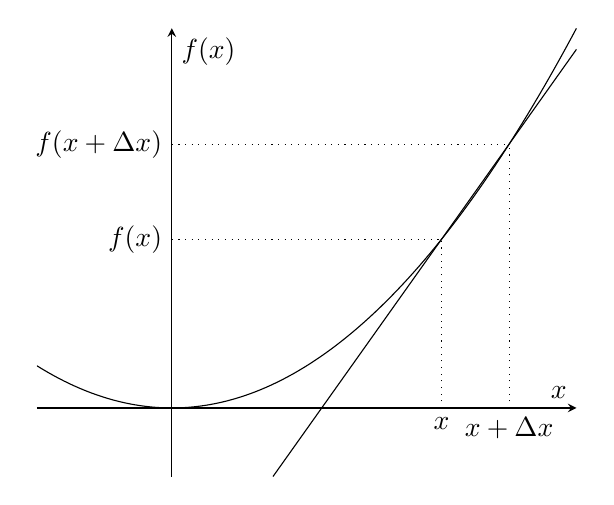
\begin{tikzpicture}[scale=1]
    \begin{axis}[
        axis lines = left,
        axis lines = center,
        xtick style={draw=none},
        ytick style={draw=none},
        xticklabels={},
        yticklabels={},
        xlabel = {$x$},
        ylabel = {$f(x)$},
    ]
    
    \node [left] at (0, 64) {\(f(x)\)};
    \node [left] at (0, 100) {\(f(x + \Delta x)\)};
    \node [below] at (8, 0) {\(x\)};
    \node [below] at (10, 0) {\(x + \Delta x\)};
    \addplot [
        domain=-4:12, 
        samples=100, 
        color=black,
    ]
    {x^2};
    \addplot+ [
        black, dotted,
        mark=none,
    ]
    coordinates {
        (8,0)
        (8,64)

        (10,0)
        (10,100)

        (0, 64)
        (8, 64)

        (0, 100)
        (10, 100)

    };
    \addplot+ [
        black,
        mark=none
    ]
    coordinates {
        (3,-26)
        (12, 136)
    };
    \end{axis}
    \end{tikzpicture}
\end{center}

Here we have two points, one at $x = x_1$ and $x = x_2 = x_1 + \Delta x$. Here $\Delta$ means "change in"
and so $\Delta x$ denotes the difference between our two x values. The corresponding function values are
$f(x_1)$ and $f(x_1 + \Delta x)$ where the difference between these two values is $\Delta f$. We can say 
a reasonable estimate of the rate of change would be the gradient of the line that passes through these two 
points. We can write this as

\begin{equation} \label{gradient}
    \frac{\Delta f}{\Delta x} = \frac{f(x + \Delta x) - f(x)}{\Delta x}
\end{equation}

We can see that this estimate for the rate of change gets better the closer the two points are, or the smaller 
$\Delta x$ gets. If we take the limit of $\Delta x \to 0$, then our two points become infinitesimally close and the
line through them becomes the tangent line to the curve. Thus we arrive at the definition of the derivative and the
idea of "instantaneous" rate of change. The derivative is defined as a function which gives us the gradient of the 
tangent line to a curve at a point $x$. Mathematically we can write this as

\begin{equation*}
    f'(x) \equiv \frac{df}{dx} \equiv \lim_{\Delta x \to 0} \frac{\Delta f}{\Delta x}\\
\end{equation*}

Using the expression for the gradient above we then get

\begin{equation} \label{deriv-def}
    \frac{df}{dx} \equiv \lim_{\Delta x \to 0} \frac{f(x + \Delta x) - f(x)}{\Delta x}
\end{equation}

Which is our formal definition of the derivative. The process of finding a functions derivative is called 
differentiation. We can differentiate from first principles using the expression above.\\

\noindent\textbf{Example: Differentiate the function $x^2$ using first principles.}

Using equation \ref{deriv-def}, we have that

\begin{align*}
    \frac{d}{dx}(x^2) &= \lim_{\Delta x \to 0} \frac{(x + \Delta x)^2 - x^2}{\Delta x}\\
    &= \lim_{\Delta x \to 0} \frac{(x^2 + 2x\Delta x + \Delta x^2) - x^2}{\Delta x}\\
    &= \lim_{\Delta x \to 0} \frac{2x\Delta x + \Delta x^2}{\Delta x}\\
    &= \lim_{\Delta x \to 0} 2x + \Delta x\\
    &= 2x\\
\end{align*}

We can generalise the above example  by differentiating $x^n$ instead. With which we get

\begin{align*}
    \frac{d}{dx}(x^{n}) &= \lim_{\Delta x \to 0} \frac{(x + \Delta x)^{n} - x^{n}}{\Delta x}\\
    &= \lim_{\Delta x \to 0} \frac{(x^{n} + n x^{n-1}\Delta x + \binom{n}{2}x^{n-2}\Delta x^{2} +\dots) - x^{n}}{\Delta x}\\
    &= \lim_{\Delta x \to 0} \frac{n x^{n-1}\Delta x + \binom{n}{2}x^{n-2}\Delta x^{2}}{\Delta x} + \dots\\
    &= \lim_{\Delta x \to 0} n x^{n-1} + \binom{n}{2}x^{n-2}\Delta x + \dots\\
    &= n x^{n-1}
\end{align*}

We know this is true for all $n$ as any subsequent terms will contain a factor of $\Delta x$ which 
follows from the binomial theorem. The expression we have just derived is known as the power rule
which we can use to differentiate any power term. There are further rules of differentiation which
will allow us to differentiate any function thrown at us.

\begin{equation*}
    \frac{d}{dx}(e^{ax}) = ae^{ax}
\end{equation*}

\section{The Chain Rule}

The first rule is the chain rule which we use to differentiate composite functions, or "functions
of functions". If we have a composite function, $f[g(x)]$, then the chain rule says the derivative
of f with respect to x can be written as

\begin{equation*}
    \frac{d}{dx}f[g(x)] = \frac{df}{dg} \frac{dg}{dx}
\end{equation*}

\section{The Product Rule}

The second rule is the product rule which tells us how to derivative products of functions. Formally, we 
ay derive this using equation \ref*{deriv-def}. If we define the product of two functions $f(x) = u(x)v(x)$,
then we can write

\begin{align*}
    f(x + \Delta x) - f(x) &= u(x + \Delta x)v(x + \Delta x) - u(x)v(x)\\
    &= u(x + \Delta x)v(x + \Delta x) - u(x + \Delta x)v(x) + u(x + \Delta x)v(x) - u(x)v(x)\\
    &= u(x + \Delta x)\left[v(x + \Delta x) - v(x)\right] + \left[u(x + \Delta x) - u(x)\right]v(x)\\
\end{align*}

and so using our definition of the derivative,

\begin{align*}
    \frac{df}{dx} &= \lim_{\Delta x \to 0} \frac{f(x + \Delta x) - f(x)}{\Delta x}\\
    &= \lim_{\Delta x \to 0} \left\{u(x + \Delta x)\left[\frac{v(x + \Delta x) - v(x)}{\Delta x}\right] + \left[\frac{u(x + \Delta x) - u(x)}{\Delta x}\right]v(x)\right\}\\
    &= u(x)\frac{dv}{dx} + \frac{du}{dx}v(x)
\end{align*}

This can be written much more neatly using prime notation which gives us,

\begin{equation*}
    f' = (uv)' = u' v + uv'
\end{equation*}

This also works for any numbers of products. Namely, if we had $f(x) = u(x)v(x)w(x)$ then,

\begin{equation*}
    f' = u'vw + uv'w + uvw'
\end{equation*}

\section{The Quotient Rule}

Like the product rule with products of functions, the quotient rule tells how to differentiate 
quotients of functions. Consider the function $f(x) = u(x)/v(x)$, the product rule tells us that

\begin{equation*}
    f' = \left(\frac{u}{v}\right)' = u\left(\frac{1}{v}\right)' + u'\left(\frac{1}{v}\right) = u\left(-\frac{v'}{v^2}\right) + \frac{u'}{v}
\end{equation*}

Combining our two fractions and we get

\begin{equation*}
    f' = \left(\frac{u}{v}\right)' = \frac{vu' - uv'}{v^2}
\end{equation*}

Which is our quotient rule.

\section{Implicit Differentiation}